%%% =====================================================================
%%% SOTA - Section 2: Structured document layouts
%%% Mirrors Chapter~\ref{chapter:template}. Addresses SO1.
%%% Treatment levels: 2.3 and 2.5 are P (pedagogical); the rest is R.
%%% =====================================================================

\section{Structured document layouts: representation, similarity and retrieval}
\label{sec:sota-retrieval}

Assigning a template to an article requires characterizing what distinguishes one template from another, which is the challenge stated in \secref{sec:challenges} as the characterization of multiple layout elements. This section reviews the literature needed to represent, compare and retrieve such templates. 

It is important to note that the literature reviewed below treats a layout as a general object, spanning floor plans, user interfaces and arbitrary documents, since that is the level at which retrieval and similarity methods have been developed and evaluated; this thesis specializes that object to the article template, a single reusable layout unit assigned to one article within a page.

\subsection{From text-centric retrieval to structured and visual document retrieval}
\label{sec:sota-sdr}

Historically, Information Retrieval (IR) treated documents as a sequence of blocks of text. The emergence of Structured Document Retrieval (SDR), however, recognized that documents are aggregates of interrelated objects with specific logical and physical structures~\cite{chiaramella-sdr-2001}. To exploit this structural information, Document Layout Analysis (DLA) serves as a critical preprocessing step that detects and labels homogeneous physical regions~\cite{binmakhashen-survey-2019}. While traditional DLA often focuses on extracting text components for Optical Character Recognition (OCR), visual-centric domains require a different perspective, in which the structure itself is the target of the search.

Unlike text-based IR, Document Image Retrieval (DIR) addresses the retrieval of entire page layouts based purely on their geometric and spatial arrangement, independently of textual content~\cite{yan-geometric-2013, vanbeusekom-distance-2006}. This is particularly relevant when keyword search falls short, whether because of language barriers, the absence of explicit text, or because the intent of the query relies on visual memory of the spatial distribution of the layout~\cite{yan-geometric-2013}, and recent literature confirms that pairwise comparison of layout geometric characteristics remains an effective mechanism to support this kind of retrieval~\cite{jaha-comparative-2024}.

\subsection{Measuring pairwise layout similarity}
\subsubsection{Intersection-over-Union and its distance-based extensions}
\label{sec:sota-geometric-similarity}

Once two layouts are represented as sets of labeled blocks, comparing them geometrically first requires a measure of overlap between individual blocks. The Intersection-over-Union ratio, also known as the Jaccard index~\cite{jaccard2021}, is the default choice: it is symmetric, bounded and invariant to block size, computed as the area of overlap divided by the area of union. Comparing complete layouts, however, means aggregating many such pairwise block comparisons rather than a single one, and the ratio inherits two limitations from its block-level definition that carry over unchanged: (1) it is sensitive to small positional misalignments, penalizing near-identical placements as if they belonged to unrelated layouts, and (2) it saturates at zero whenever two blocks do not overlap at all, which no longer distinguishes a near-miss from a placement in opposite corners of the page and offers no usable gradient to an optimization procedure, for example. 

The object detection literature, where Intersection-over-Union is used both as an evaluation metric and as a training loss, has proposed two corrections to the second limitation. Generalized IoU~\cite{Rezatofighi_2019_CVPR} restores a usable signal for non-overlapping blocks by subtracting, from the plain ratio, the share of the smallest enclosing block that is covered by neither of the two compared blocks; the resulting measure decreases smoothly as two blocks move further apart, even before they touch. Distance-IoU~\cite{zheng_distance-iou_2019} pursues the same goal along a different path, adding to the ratio a term proportional to the normalized distance between block centers, which converges faster in practice and further penalizes centers that drift apart even when the enclosing block already covers both blocks.

Extending any of these block-level measures to entire layouts additionally requires deciding which block of one layout corresponds to which one of the other before their similarities can be aggregated. When blocks are typed and each one admits at most one counterpart, this correspondence is an instance of the assignment problem, classically solved to optimality by the Hungarian algorithm~\cite{hungarian}, which finds the pairing that maximizes total matched similarity in polynomial time.

Even under an optimal assignment, however, the resulting layout-level score remains a sum of independently computed block-level comparisons: it reflects how well each matched pair of blocks overlaps, but not how the matched elements relate to one another. This motivates the usage of graph-structures to model layouts.

\subsubsection{Graph matching networks to measure similarity between layouts}
\label{sec:sota-gmn}

Layout templates are complex structures defined by the relative context between their inner elements, such as distances and relative orientations between images, captions and titles, rather than by absolute coordinates. Their topology is therefore best captured through graph representations, in which nodes denote content blocks and edges denote spatial or hierarchical relationships. Graph Neural Networks (GNNs) have emerged as the standard framework for encoding this kind of relational data, and Graph Matching Networks~\cite{li-gmn-2019} in particular replace independently computed graph embeddings with a joint, cross-graph reasoning mechanism specifically suited to comparing near-identical structures.

\paragraph{Graph neural networks}
A graph $G=(V,E)$ consists of a set of nodes $V$ and a set of edges $E$ connecting them; each node $i \in V$ may carry a feature vector $x_i$, and each edge $(i,j) \in E$ a feature vector $x_{ij}$. A GNN computes a representation for such a graph in three stages~\cite{li-gmn-2019}. An encoder first maps the raw node and edge features to initial node embeddings $h_i^{(0)}$ through a small feed-forward network. A sequence of propagation layers then updates every node embedding by aggregating messages from its neighbors: at propagation step $t$, a message $m_{j\to i}$ is computed for every edge $(j,i)\in E$ as a function of the current embeddings of both endpoints and of the edge features, and the embedding of node $i$ is updated from its previous embedding and the sum of the incoming messages. After a fixed number of such rounds, node embeddings encode information aggregated over an increasingly large neighborhood. Finally, an aggregator pools the set of node embeddings into a single graph-level embedding, typically through a weighted sum whose weights are themselves learned, so that irrelevant nodes contribute less to the final representation.

\paragraph{From graph embedding to graph matching}
Applied to a pair of graphs $G_1$ and $G_2$, a GNN of this kind embeds each of them independently into a vector, after which similarity is measured by a standard distance in that vector space; this is a \emph{graph embedding model}. Because the two graphs never interact during encoding, subtle structural differences between two otherwise near-identical layouts are easy to lose, as whatever an embedding does not preserve cannot be recovered afterwards by any downstream distance computation~\cite{li-gmn-2019}. \emph{Graph Matching Networks} (GMNs) address this by computing the two embeddings jointly rather than independently, letting each graph condition its representation on the other throughout propagation. 

\paragraph{Cross-graph attention}
A GMN modifies the propagation layer of a graph embedding model by adding, alongside the intra-graph messages $m_{j\to i}$, a cross-graph matching vector that measures how well a node in one graph is matched by the nodes of the other. For a node $i$ in $G_1$, this vector aggregates a cross-graph term $\mu_{j\to i}$ computed against every node $j$ in $G_2$:
\[
a_{j\to i} = \frac{\exp\!\left(s_h\!\left(h_i^{(t)}, h_j^{(t)}\right)\right)}{\sum_{j'} \exp\!\left(s_h\!\left(h_i^{(t)}, h_{j'}^{(t)}\right)\right)}, \qquad
\mu_{j\to i} = a_{j\to i}\left(h_i^{(t)} - h_j^{(t)}\right),
\]
where $s_h$ is a vector-space similarity such as the dot product, and the attention weights $a_{j\to i}$ are normalized over all nodes of the other graph~\cite{li-gmn-2019}. The node embedding is then updated from its previous value, the intra-graph messages, and the sum $\sum_j \mu_{j\to i}$, which has a direct interpretation: it is the difference between $h_i^{(t)}$ and its closest match in the other graph, weighted by the attention distribution. When the two graphs are structurally identical and every node finds a perfect counterpart, this sum collapses to zero and both graphs continue to compute identical representations under further propagation; whenever a structural difference exists, the corresponding node keeps producing a nonzero cross-graph term, which is then amplified across subsequent propagation rounds. The final graph-level embeddings are obtained by the same aggregator as in the embedding model, and the pair is compared with the same vector-space similarity.

\paragraph{Triplet-based metric learning}
Both graph embedding and graph matching models are trained as similarity metrics rather than classifiers, using pairs or triplets of graphs. In the triplet setting, each training example consists of an anchor graph $G_1$, a positive graph $G_2$ known to be more similar to the anchor than a negative graph $G_3$, and the network is trained with a margin-based triplet loss:
\[
\mathcal{L}_{\text{triplet}} = \mathbb{E}_{(G_1,G_2,G_3)}\left[\max\left(0,\; d(G_1,G_2) - d(G_1,G_3) + \gamma\right)\right],
\]
where $d(\cdot,\cdot)$ is the distance between the learned graph embeddings and $\gamma>0$ is a margin~\cite{li-gmn-2019}. Because the loss depends only on the relative ordering of the two distances, this formulation requires only relative similarity judgments rather than an absolute ground-truth similarity value for every pair, which makes it possible to train on weak labels, that is, on proxy signals obtained without human annotation that are only assumed to correlate with true similarity rather than to define it exactly.

\paragraph{LayoutGMN} 
Patil et al.~\cite{patil_layoutgmn_2021} instantiate this triplet-based framework for layout data, under the name LayoutGMN, representing each layout, whether a floor plan, a user interface, or a document, as a directed, fully connected graph over its constituent blocks. Every node encodes the geometric position and size of one element together with its semantic type, and every edge encodes the relative position, aspect ratio, and Intersection-over-Union between the two blocks it connects. Because reliable ground-truth similarity between layouts is expensive to obtain, and subjective human judgments over structured data are known to disagree even among domain experts, LayoutGMN is trained with weak labels obtained purely from Intersection-over-Union: a candidate layout is treated as a positive example above one IoU threshold against a query layout, and as a negative example once its IoU falls sufficiently below that threshold. On its own, this weak-supervision strategy inherits the two limitations of Intersection-over-Union described in \secref{sec:sota-geometric-similarity}, since the metric used to construct the labels is the same one the network is meant to improve upon.

What makes the resulting metric structurally aware, despite being trained from purely geometric labels, is the structural bias introduced by cross-graph attention. Because each node in one layout adjusts its representation against every node of the other, the network is forced to reason about which elements correspond to which, rather than only about how much of the page they cover. Patil et al.\ report that this bias can be strong enough to overturn the Intersection-over-Union labels the network was trained on: two layouts that Intersection-over-Union would label as dissimilar, because their elements sit in different absolute positions, can be predicted as clearly more structurally similar than a layout Intersection-over-Union would rate positively, whenever the two share more of their underlying topology~\cite{patil_layoutgmn_2021}. In retrieval experiments over large floor plan and interface datasets, results returned under the learned metric matched crowd-sourced human judgments of structural similarity more closely than either Intersection-over-Union directly or a competing graph-embedding baseline, confirming that the network generalizes beyond the geometric signal used to supervise it.

Given the advantages of LayoutGMN as a deep graph-based method to compute similarity, this thesis adapts it directly (\secref{section:modelling-similarity}): article templates are represented as graphs following the same principles, and the resulting cross-graph matching vectors are turned into the bounded similarity metric used throughout Chapter~\ref{chapter:template} for template retrieval.


\begin{figure}[htbp]
    \centering
     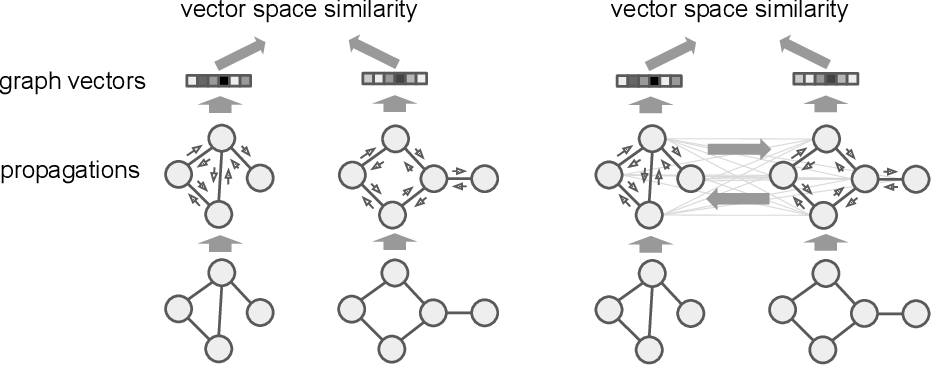
\includegraphics[width=\widthForOneImage]{img/gmn-embedding-vs-matching.png}
    \caption{Graph embedding models, which encode each graph independently, compared with graph matching models, which compute both embeddings jointly through cross-graph attention. Adapted from Figure~2 of~\protect\cite{li-gmn-2019}.}
    \label{fig:sota-gmn-architecture}
\end{figure}

\begin{figure}[htbp]
    \centering
     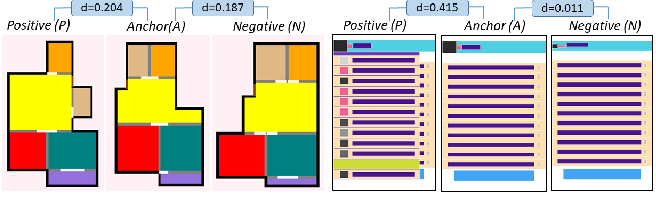
\includegraphics[width=\widthForOneImage]{img/layoutgmn-neutralizes-iou.png}
    \caption{Structural bias overturning Intersection-over-Union labels: a layout pair labeled ``negative'' by IoU thresholding is predicted as more structurally similar by LayoutGMN than a pair labeled ``positive'', because the two share more of their underlying topology. Adapted from Figure~2 of~\protect\cite{patil_layoutgmn_2021}.}
    \label{fig:sota-layoutgmn-neutralize}
\end{figure}

\begin{figure}[htbp]
    \centering
     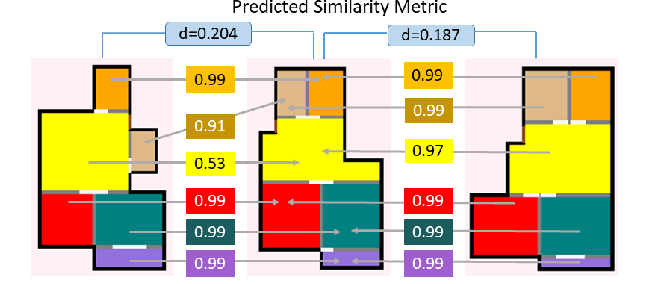
\includegraphics[width=0.7\widthForOneImage]{img/layoutgmn-attention.png}
    \caption{Attention-based element correspondence learned by LayoutGMN between a query layout and a retrieved result. Adapted from Figure~1 of~\protect\cite{patil_layoutgmn_2021}.}
    \label{fig:sota-layoutgmn-triplet}
\end{figure}


\subsection{Beyond pairwise similarity: diversity and novelty in retrieval}


\subsubsection{Diversity and Novelty}
\label{sec:sota-diversity}

The similarity measures reviewed above solve a pairwise problem, namely how similar two layouts are to one another. Retrieval instead compiles a small candidate set from which an editor selects the layout used for one article. The usefulness of that set depends on how much its members differ from each other, in addition to how closely each one matches the query. Constructing such a set therefore raises two concerns distinct from pairwise similarity: the diversity of the retrieved candidates, and their novelty, understood as exposure to long-tail, underused designs. These are general concepts in the Information Retrieval and Recommender Systems literature, not specific to layout retrieval.

\paragraph*{Diversity}
While the conceptualization of diversity varies across the literature~\cite{vrijenhoek-diversity-2024}, recent works unifies these efforts by defining that diversity seeks structural variety within the retrieved set~\cite{clarke-2008}. Achieving such variety requires solving a bi-criterion optimization problem that balances diversity against conflicting relevance objectives, such as conformity to historical usage~\cite{javari-div}. To navigate this trade-off, clustering-based methods are frequently employed, as they span the structural range of the dataset efficiently without compromising relevance~\cite{clustering-survey, zheng-survey-2017, akinyemi-diversity-2012, divsurvey}. Applied to a catalog of structured layouts, this trade-off translates into balancing how closely a candidate matches the query template against how much its underlying structure differs from the other candidates already returned~\cite{zheng-survey-2017}.

\paragraph*{Novelty}
Novelty, in contrast, aims to avoid redundancy by exposing users to new, less obvious, or \emph{long-tail} items~\cite{clarke-2008, wu-survey-2022}. This notion is grounded in how item usage is typically distributed: usage in such catalogs follows a power-law distribution, in which a ``short-head'' subset dominates interactions while a ``long-tail'' remains underutilized, a pattern often referred to as the ``super-star'' economy in recommender systems~\cite{wu-survey-2022} and documented both in the deep learning domain~\cite{longtail-deep} and in the recommender systems literature~\cite{longtail}. This imbalance produces a severe popularity bias and a cold-start problem for tail items, limiting the effective variety of the system and obscuring valuable but unpopular design options~\cite{longtail}, which novelty-promoting mechanisms aim to surface while ensuring fair catalogue exposure~\cite{wu-survey-2022}. A common methodology involves clustering-based strategies: Park and Tuzhilin~\cite{long-tail-ei-tc} employed item grouping to improve tail visibility, while more recent adaptive approaches refine this method by defining head-tail boundaries dynamically from real-time data~\cite{longtail-clustering-based}. Graph-based~\cite{graphmethod-1, graphmethod-2, graphmethod-3} and deep learning~\cite{dl-1, dl-2, dl-3, dl-4} formulations of the same problem have also been proposed. Applied to a catalog of structured layouts, the same short-head pattern means that a small subset of designs dominates historical usage, leaving structurally distinct templates effectively invisible to any retrieval mechanism that only reinforces past popularity.

\subsubsection{A specific algorithm for diversity-based retrieval: ClusDiv}
\label{sec:sota-clusdiv}


One instantiation of the clustering-based strategies described above is ClusDiv~\cite{clusdiv}, whose notation and cluster-weight mechanism are reused directly in \secref{section:template-retrieval-single-article}.

ClusDiv operates in two phases. 
\begin{itemize}
    \item \textbf{Offline: }the item catalog is partitioned into $N$ clusters $C = \{C_1, \dots, C_N\}$ using $k$-means over historical rating data, where $N$ is fixed to the size of the target recommendation list; no content information about the items is used at this stage.
    \item \textbf{Online: }given a user $u$ and the top-$N$ list $L_0(u)$ produced by an underlying prediction algorithm (for example, collaborative filtering~\cite{cf-techniques}), ClusDiv redistributes that list across clusters through a set of cluster weights $CW$, whose entry $CW_{ui}$ counts how many items cluster $C_i$ contributes to the final list of user $u$, subject to $\sum_i CW_{ui} = N$.
\end{itemize}

Cluster weights are computed in two steps. 

\begin{enumerate}
    \item They are initialized from the original ranking,
        \[
        CW_{ui} = |C_i \cap L_0(u)|,
        \]
        that is, the number of items from the unmodified top-$N$ list that fall in cluster $C_i$. 

    \item Then, each weight is redistributed away from any cluster whose count exceeds a fixed threshold: while $CW_{ui} > \text{threshold}$, one unit is moved from cluster $i$ to the cluster $c$ currently holding the smallest weight, $c = \arg\min_j CW_{uj}$, updating $CW_{uc} \mathrel{+}= 1$ and $CW_{ui} \mathrel{-}= 1$.  This threshold is the only tunable parameter of the method: as it approaches $N$, no redistribution occurs and the original ranking is preserved; smaller values force weight into a larger number of clusters, trading relevance for diversity.
\end{enumerate}


Once the final weights are fixed, the diversified list is assembled by scanning the ranked list (based on the underlying prediction algorithm), admitting an item whenever the weight of its cluster is still positive and decrementing that weight, until every cluster weight reaches zero.

However, this type of clustering-method operates entirely on rating: items are grouped by how similarly they have been rated, and the number of clusters is tied to the size of the output list, not to any independent measure of catalog variety. Two items with markedly different visual or structural properties can therefore fall into the same cluster purely because they were rated similarly, and, conversely, near-identical items can be split across clusters because of differences in usage. This coupling between cluster granularity and list size, together with the reliance on rating-based rather than content-based grouping, is the departure point for the adaptation used in \secref{section:template-retrieval-single-article}.


\subsection{Beyond independent retrieval: context-aware scoring of joint item sets}
\label{sec:sota-page-aware-scoring}

%%% -----------------------------------------------------------------
%%% STRUCTURE STILL TENTATIVE. This subsection positions \neuralmethod, a Transformer
%%% encoder that scores template assignments jointly over all articles of a page and
%%% is consumed as an objective in \secref{sec:sota-pagegen}. The previous paper had no
%%% state of the art for it (see the note formerly in template/sections/sota.tex).
%%% Four candidate entry points are proposed below, with search keywords, so that the
%%% literature can be gathered before deciding whether this stays as one subsection
%%% or is split in two.
%%%
%%% (1) Transformers as set encoders. Self-attention~\cite{attention} over a set of
%%%     articles. A page is a SET, not a sequence: this must be argued or refuted
%%%     explicitly. Keywords: set transformer / deep sets / permutation invariant
%%%     neural network / set-input neural architecture.
%%% (2) Neural layout generation and assessment. Keywords: layout generation
%%%     transformer / conditional layout generation / document layout synthesis deep
%%%     learning / layout quality assessment / neural design scoring / computational
%%%     design aesthetics.
%%% (3) Recommending coherent sets. Choosing templates that work well TOGETHER on a
%%%     page is formally analogous to recommending a set rather than independent items.
%%%     Considered the most promising framing. Keywords: slate recommendation / bundle
%%%     recommendation / complementary item recommendation / set-aware recommendation /
%%%     basket completion.
%%% (4) Classification over large catalogues with long-tailed label distributions,
%%%     connecting back to~\cite{longtail-deep}. Keywords: extreme multi-label
%%%     classification / long-tailed classification / label distribution skew.
%%% -----------------------------------------------------------------

%%% REFGAP: this subsection has essentially no coverage in the current bibliography.

\subsection{Positioning and open gaps}
\label{sec:sota-retrieval-gaps}

%%% TODO[SOTA]: to be written. The gaps to state, each already prepared above:
%%%  (a) Layout retrieval has been addressed with hand-designed geometric heuristics or
%%%      strict coordinate matching, whereas the structural comparison required here is
%%%      learned. This motivates representing templates as graphs and using a GNN-based
%%%      pairwise comparison (\secref{sec:sota-gmn}).
%%%  (b) Clustering-based diversification defines diversity over usage statistics rather
%%%      than over structure (\secref{sec:sota-clusdiv}), so it cannot guarantee that the
%%%      returned candidates are genuinely distinct designs. Shifting the clustering
%%%      distance from usage frequency to structural difference unifies both goals:
%%%      intrinsic structural diversity, and novelty through the exposure of underused
%%%      long-tail templates.
%%%  (c) No existing system scores template assignments jointly at page level
%%%      (\secref{sec:sota-page-aware-scoring}).
%%% Close by naming Chapter~\ref{chapter:template} and the first specific objective.
